\chapter{Experiments}
In this chapter, I describe the details about the two different experiments.
These experiments should demonstrate the way how such a system can monitor and analyze the development in order to improve it and find weaknesses.\\
The goal of the first one is to to find correlations between the data gathered from the mobile devices and the code quality. The second experiments purpose is to find individual factors that influence the cognitive performance of a single person. \\
This chapter shows the execution of the experiments as well as the usage of the gathered data and how the data is been interpreted. 

\section{Group Experiment}

\begin{figure}
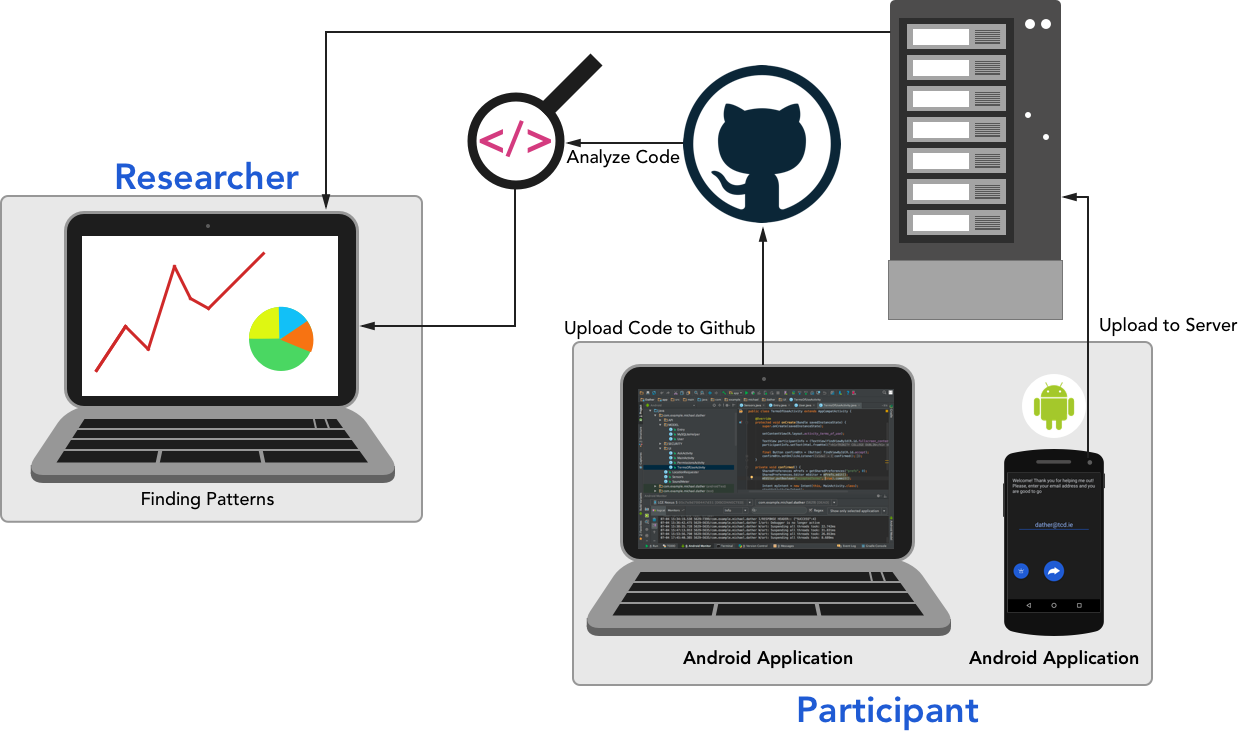
\includegraphics[width=\textwidth]{experiment}
\caption{Experiment Execution}\label{experiment}
\vspace{10 mm}
\end{figure}

Five participants solved a programming task while the mobile application was gathering the environment and working patterns. 
After completion, they submitted the gathered data to our server and deployed their solution in a public Github repository. 
An overview of the experiment procedure is shown in figure \ref{result}.
 
\subsection{Setup and Execution}
Every participant needed to install the 'Dather' app on a mobile phone with at least Android version 4.4.  
They downloaded the app from the project website \footnote{\url{http://frickm.de}} by accessing the URL from the Android device. The website also provided information about the setup and usage of the application. 
\bigbreak
At the first start, after installing the downloaded app, the participants needed to login with his/her Github username, followed by granting the permissions to use the sensors and access the required device information.\\
After setting up the application the experiment is ready to start. 
The participant runs the gathering process while working on the programming task as described in the next section .\\
After completing, the participants uploaded their solution code to Github and provided a link of the Github repository to the research team. The Github account name was later be used to match the gathered data with the uploaded solution-code of the participant. 

\subsection{Programming Task}
The programming task for the participants has been provided via the project website \footnote{\url{http://www.frickm.de/codingTask.html}}. 
The Participants were asked to create a solution to calculate the number of character from a string, that can not be used to create a palindrome  \footnote{A palindrome is a word which reads the same from left to right and right to left such as anna or racecar}.
The whole programming task with examples can be found in the appendix of this dissertation. 
The participants could use their favorite programming language to address the problem while they let the android application gather their data. 
\bigbreak
The experiment showed that the participants had some issues understanding the explanation of the problem. The example brought clarity and helped to understand but wasted time of the participants who partially read the question and the next steps while they were working on the task.  
 
\section{Individual Experiment}
The purpose of the second experiment is to find evidence of specific factors that influence the ability of cognitive thinking. Different isolated scenarios are been tested by a participant in order to find correlations between the specific environments. 
This experiment allows to test the factors in a more controllable environment but based on one individual person. 

\subsection{Setup and Execution}
In this experiment a participant solved some cognitive tasks while being in a controlled environment in order to test the performance influences of isolated factors. 
Of course it is very unlikely or even impossible to test a factor in complete isolation one factor. There are always side factors that which are unavoidable. They could be for example the human itself, sudden unpredictable changes in the environment and of course the problem in keeping the factors of one part of the measurement equal to the factors of other measurements. 
To minimize these factors, the 'Dather' Android application helped to monitor the environment and remove recorded tasks where the environment information are too different of results which are were correlated with each other. 
However, with this problems in mind, the idea to measure changes in the cognitive performance of a person, was measuring the time of finishing a Sudoku game. 
The game, where the goal is to systematically add missing numbers in a 9x9 matrix, requires concentration and logical combining of numbers. 
The sudoku game was already used in previous research for measuring the cognitive performance \cite{sobolewski2009monitoring} \cite{xiang2009using}. 
Another reason for using Sudokus is that they can be randomly generated with a specific calculated difficulty level to make sure that every Sudoku is equally hard to solve. 
A website \footnote{\url{http://www.opensky.ca/~jdhildeb/software/sudokugen}} generated the Sudokus uses an engine which is part of the gnome-sudoku software \footnote{\url{https://sourceforge.net/projects/gnome-sudoku}}. 
A medium difficulty level and a limited calculated range of difficulty to +/- 0.02 of 0.5 was the base for generating the Sudokus which were then printed on paper, one per page. 

\subsection{Scenarios}
The following scenarios have been tested. Each scenario was performed 10 times to get a good mean which decreases the randomness in the experiment. In order to control the environment variables, a modified version of the Android app recorded the environmental light and volume and it was made sure that the values don't differ much to have a influence in the results. 
The experiments were executed over a several days in mixed up order to avoid that the training-process in solving the Sudokus can also influence the overall average of the outcomes.

\subsubsection{Music}
The scenarios to compare in this part the influence of two different types of music and as a control scenario no music at all. The participant did the Sudokus while listening to Spotify-Radio \footnote{\url{https://www.spotify.com}} 'Heavy Metal' and 'Classical' over headphones on a defined level of volume. In the control case without music, the participant was not wearing headphone but working in a very quite environment.

\subsubsection{Coffee}
In this scenario I wanted to test the influences of Coffee in the cognitive performance as discovered by Watters, Paul Andrew et. al. \cite{watters1997caffeine}. Simultaneously to their results I used a caffeine level of almost the value that they found out is the optimum for cognitive performance (400 mg). 
The whole experiment was executed in 5 days in a row with two tasks before, and two tasks after having a coffee. 
First, the participant solved the Sudokus without taking any caffeine for more than 16 hours, which is more than enough to make sure no other caffeine intake can influence to experiment \cite{liguori1997absorption}. Additionally the participant had the same breakfast every day before every experiment. 
For the second part of the experiment, the participant had the coffee drink. The Coffee Franchise declares one espresso with 75mg caffeine each, which sums our drink up to 375mg at an amount of 5. After having the coffee, the participant waited 40 minutes for the caffeine to be absorbed \cite{liguori1997absorption} and started with the Sudoku. 

\subsubsection{Running}
This scenario compares the Sudoku result from before and after running for 30 minutes at a speed of 10 kph in a gym. 10 minutes break are between finishing the run the beginning of solving the Sudoku. The 10 kph for 30 minutes was a duration which was very exhausting for the participant during the test. 
Hillman C, et al. \cite{hillman2008smart} found evidence for long term improvement of the cognitive ability now I want to find out how activity up to a level of exhaustion influences the brain performance. A possibility would be an increase of the performance related to the supply of more blood and oxygen while the heart beat is significantly faster during activity it would also be possible that the exhausted body enters a state to save energy after high activity and decreases the energy and heart rate. 

\section{Summary}
Three experiments are described in this section. The first experiment gathers data while participants work on a programming task. 
Second, a participant is solving 10 Soduku riddles for each isolated environment (normal vs. after drinking 375 ml caffeine, silence vs. classical music vs. heavy metal, normal vs. after running for 30 min) and being compared to the its counter parts. 
